
\section{Creative performance analysis}
\label{appendix:creative_performance_analysis}

\subsection{Return on Advertising Spend (ROAS)}
\label{appendix:creative_performance_analysis_ROAS}

\subsubsection{Descriptive Statistics}

\begin{table}[H]
	\centering
	\caption{Descriptive statistics for ROAS by creative type.}
	\begin{tabular}{lcccc}
		\toprule
		Creative Type & Mean & Median & Std. Dev. & Count \\
		\midrule
		Carousel & 0.7560 & 0.6572 & 0.4480 & 355 \\
		Display & 0.6626 & 0.6194 & 0.2685 & 348 \\
		Image & 0.6176 & 0.5656 & 0.2749 & 349 \\
		Search & 1.3244 & 1.2455 & 0.6708 & 705 \\
		Video & 0.9886 & 0.9058 & 0.4730 & 1416 \\
		\bottomrule
	\end{tabular}
\end{table}

\subsubsection{Assumption Tests}

\subsubsection{Shapiro--Wilk Test}

\begin{table}[H]
	\centering
	\begin{tabular}{lc}
		\toprule
		Creative Type & p-value \\
		\midrule
		Carousel & $<0.0001$ \\
		Display & $<0.0001$ \\
		Image & $<0.0001$ \\
		Search & $<0.0001$ \\
		Video & $<0.0001$ \\
		\bottomrule
	\end{tabular}
\end{table}

All creative type distributions significantly deviated from normality ($p<0.05$).

\vspace{0.3cm}

\subsubsection{Levene's Test}

\begin{table}[H]
	\centering
	\begin{tabular}{lc}
		\toprule
		Statistic & Value \\
		\midrule
		p-value & $<0.0001$ \\
		\bottomrule
	\end{tabular}
\end{table}

The variability of \textbf{ROAS differed significantly} across creative types.

\vspace{0.3cm}

\subsubsection{Kruskal--Wallis Test}

\begin{table}[H]
	\centering
	\begin{tabular}{lc}
		\toprule
		Statistic & Value \\
		\midrule
		H-statistic & 606.8404 \\
		p-value & $<0.0001$ \\
		\bottomrule
	\end{tabular}
\end{table}

The Kruskal--Wallis test indicates statistically significant differences in ROAS across creative types.

\vspace{0.3cm}

\subsubsection{Dunn Post-hoc Test}

\begin{table}[H]
	\centering
	\caption{Pairwise Dunn test p-values (Bonferroni adjusted).}
	\begin{tabular}{lccccc}
		\toprule
		& Carousel & Display & Image & Search & Video \\
		\midrule
		Carousel & -- & 0.2527 & 0.0008 & $<0.0001$ & $<0.0001$ \\
		Display & 0.2527 & -- & 0.8940 & $<0.0001$ & $<0.0001$ \\
		Image & 0.0008 & 0.8940 & -- & $<0.0001$ & $<0.0001$ \\
		Search & $<0.0001$ & $<0.0001$ & $<0.0001$ & -- & $<0.0001$ \\
		Video & $<0.0001$ & $<0.0001$ & $<0.0001$ & $<0.0001$ & -- \\
		\bottomrule
	\end{tabular}
\end{table}

\subsubsection{Summary}

\begin{itemize}
	\item The highest average ROAS was achieved by \textbf{Search} (1.3244).
	\item The lowest average ROAS was observed for \textbf{Image} (0.6176).
	\item \textbf{Search differed significantly} from all other creative types. No statistically significant differences were observed between \textbf{Carousel and Display}, or between \textbf{Display and Image}.
\end{itemize}


\subsection{Click-Through Rate (CTR)}\label{appendix:creative_performance_analysis_CTR}

\subsubsection{Descriptive Statistics}

\begin{table}[H]
	\centering
	\caption{Descriptive statistics for CTR by creative type.}
	\begin{tabular}{lcccc}
		\toprule
		Creative Type & Mean & Median & Std. Dev. & Count \\
		\midrule
		Carousel & 0.0054 & 0.0051 & 0.0021 & 355 \\
		Display & 0.0100 & 0.0098 & 0.0054 & 348 \\
		Image & 0.0055 & 0.0052 & 0.0022 & 349 \\
		Search & 0.0100 & 0.0099 & 0.0050 & 705 \\
		Video & 0.0063 & 0.0061 & 0.0018 & 1416 \\
		\bottomrule
	\end{tabular}
\end{table}

\subsubsection{Assumption Tests}

\subsubsection{Shapiro--Wilk Test}

\begin{table}[H]
	\centering
	\begin{tabular}{lc}
		\toprule
		Creative Type & p-value \\
		\midrule
		Carousel & $<0.0001$ \\
		Display & $<0.0001$ \\
		Image & $<0.0001$ \\
		Search & $<0.0001$ \\
		Video & $<0.0001$ \\
		\bottomrule
	\end{tabular}
\end{table}

All creative type distributions significantly deviated from normality ($p<0.05$).

\vspace{0.3cm}

\subsubsection{Levene's Test}

\begin{table}[H]
	\centering
	\begin{tabular}{lc}
		\toprule
		Statistic & Value \\
		\midrule
		p-value & $<0.0001$ \\
		\bottomrule
	\end{tabular}
\end{table}

The variability of \textbf{CTR differed significantly} across creative types.

\vspace{0.3cm}

\subsubsection{Kruskal--Wallis Test}

\begin{table}[H]
	\centering
	\begin{tabular}{lc}
		\toprule
		Statistic & Value \\
		\midrule
		H-statistic & 658.6765 \\
		p-value & $<0.0001$ \\
		\bottomrule
	\end{tabular}
\end{table}

The Kruskal--Wallis test indicates statistically significant differences in CTR across creative types.

\vspace{0.3cm}

\subsubsection{Dunn Post-hoc Test}

\begin{table}[H]
	\centering
	\caption{Pairwise Dunn test p-values (Bonferroni adjusted).}
	\begin{tabular}{lccccc}
		\toprule
		& Carousel & Display & Image & Search & Video \\
		\midrule
		Carousel & -- & $<0.0001$ & 1.0000 & $<0.0001$ & $<0.0001$ \\
		Display & $<0.0001$ & -- & $<0.0001$ & 1.0000 & $<0.0001$ \\
		Image & 1.0000 & $<0.0001$ & -- & $<0.0001$ & $<0.0001$ \\
		Search & $<0.0001$ & 1.0000 & $<0.0001$ & -- & $<0.0001$ \\
		Video & $<0.0001$ & $<0.0001$ & $<0.0001$ & $<0.0001$ & -- \\
		\bottomrule
	\end{tabular}
\end{table}

\subsubsection{Summary}

\begin{itemize}
	\item The highest average CTR was achieved by \textbf{Display} (0.0100), closely followed by \textbf{Search} (0.0100).
	\item The lowest average CTR was observed for \textbf{Carousel} (0.0054).
	\item Display and Search did not differ significantly, while Carousel and Image also showed no statistically significant difference. All remaining pairwise comparisons were statistically significant.
\end{itemize}

\subsection{Conversion Rate (CVR)}\label{appendix:creative_performance_analysis_CVR}

\subsubsection{Descriptive Statistics}

\begin{table}[H]
	\centering
	\caption{Descriptive statistics for CVR by creative type.}
	\begin{tabular}{lcccc}
		\toprule
		Creative Type & Mean & Median & Std. Dev. & Count \\
		\midrule
		Carousel & 0.0300 & 0.0289 & 0.0078 & 355 \\
		Display & 0.0178 & 0.0169 & 0.0054 & 310 \\
		Image & 0.0265 & 0.0252 & 0.0081 & 349 \\
		Search & 0.0291 & 0.0284 & 0.0066 & 644 \\
		Video & 0.0264 & 0.0266 & 0.0079 & 1416 \\
		\bottomrule
	\end{tabular}
\end{table}

\subsubsection{Assumption Tests}

\subsubsection{Shapiro--Wilk Test}

\begin{table}[H]
	\centering
	\begin{tabular}{lc}
		\toprule
		Creative Type & p-value \\
		\midrule
		Carousel & $<0.0001$ \\
		Display & $<0.0001$ \\
		Image & $<0.0001$ \\
		Search & $<0.0001$ \\
		Video & 0.0001 \\
		\bottomrule
	\end{tabular}
\end{table}

All creative type distributions significantly deviated from normality ($p<0.05$).

\vspace{0.3cm}

\subsubsection{Levene's Test}

\begin{table}[H]
	\centering
	\begin{tabular}{lc}
		\toprule
		Statistic & Value \\
		\midrule
		p-value & $<0.0001$ \\
		\bottomrule
	\end{tabular}
\end{table}

The variability of \textbf{CVR differed significantly} across creative types.

\vspace{0.3cm}

\subsubsection{Kruskal--Wallis Test}

\begin{table}[H]
	\centering
	\begin{tabular}{lc}
		\toprule
		Statistic & Value \\
		\midrule
		H-statistic & 489.5054 \\
		p-value & $<0.0001$ \\
		\bottomrule
	\end{tabular}
\end{table}

The Kruskal--Wallis test indicates statistically significant differences in CVR across creative types.

\vspace{0.3cm}

\subsubsection{Dunn Post-hoc Test}

\begin{table}[H]
	\centering
	\caption{Pairwise Dunn test p-values (Bonferroni adjusted).}
	\begin{tabular}{lccccc}
		\toprule
		& Carousel & Display & Image & Search & Video \\
		\midrule
		Carousel & -- & $<0.0001$ & $<0.0001$ & 1.0000 & $<0.0001$ \\
		Display & $<0.0001$ & -- & $<0.0001$ & $<0.0001$ & $<0.0001$ \\
		Image & $<0.0001$ & $<0.0001$ & -- & $<0.0001$ & 1.0000 \\
		Search & 1.0000 & $<0.0001$ & $<0.0001$ & -- & $<0.0001$ \\
		Video & $<0.0001$ & $<0.0001$ & 1.0000 & $<0.0001$ & -- \\
		\bottomrule
	\end{tabular}
\end{table}

Carousel and Search did not differ significantly, while Image and Video also showed no statistically significant difference. All remaining pairwise comparisons were statistically significant.

\subsubsection{Summary}

\begin{itemize}
	\item The \textbf{highest average CVR} was achieved by \textbf{Carousel} (0.0300), closely followed by \textbf{Search} (0.0291).
	\item The \textbf{lowest average CVR} was observed for \textbf{Display} (0.0178).
	\item Carousel and Search exhibited statistically similar CVRs, while Image and Video also did not differ significantly. All other pairwise comparisons showed statistically significant differences.
\end{itemize}



\subsection{Cost Per Click (CPC)}\label{appendix:creative_performance_analysis_CPC}

\subsubsection{Descriptive Statistics}

\begin{table}[H]
	\centering
	\caption{Descriptive statistics for CPC by creative type.}
	\begin{tabular}{lcccc}
		\toprule
		Creative Type & Mean & Median & Std. Dev. & Count \\
		\midrule
		Carousel & 3.0715 & 2.6470 & 1.4731 & 355 \\
		Display & 1.8540 & 1.5707 & 0.9053 & 310 \\
		Image & 3.0082 & 2.6030 & 1.4140 & 349 \\
		Search & 1.8847 & 1.6315 & 0.9092 & 644 \\
		Video & 2.0942 & 1.9452 & 0.7485 & 1416 \\
		\bottomrule
	\end{tabular}
\end{table}

\subsubsection{Assumption Tests}

\subsubsection{Shapiro--Wilk Test}

\begin{table}[H]
	\centering
	\begin{tabular}{lc}
		\toprule
		Creative Type & p-value \\
		\midrule
		Carousel & $<0.0001$ \\
		Display & $<0.0001$ \\
		Image & $<0.0001$ \\
		Search & $<0.0001$ \\
		Video & $<0.0001$ \\
		\bottomrule
	\end{tabular}
\end{table}

All creative type distributions significantly deviated from normality ($p<0.05$).

\vspace{0.3cm}

\subsubsection{Levene's Test}

\begin{table}[H]
	\centering
	\begin{tabular}{lc}
		\toprule
		Statistic & Value \\
		\midrule
		p-value & $<0.0001$ \\
		\bottomrule
	\end{tabular}
\end{table}

The variability of \textbf{CPC differed significantly} across creative types.

\vspace{0.3cm}

\subsubsection{Kruskal--Wallis Test}

\begin{table}[H]
	\centering
	\begin{tabular}{lc}
		\toprule
		Statistic & Value \\
		\midrule
		H-statistic & 409.9110 \\
		p-value & $<0.0001$ \\
		\bottomrule
	\end{tabular}
\end{table}

The Kruskal--Wallis test indicates statistically significant differences in CPC across creative types.

\vspace{0.3cm}

\subsubsection{Dunn Post-hoc Test}

\begin{table}[H]
	\centering
	\caption{Pairwise Dunn test p-values (Bonferroni adjusted).}
	\begin{tabular}{lccccc}
		\toprule
		& Carousel & Display & Image & Search & Video \\
		\midrule
		Carousel & -- & $<0.0001$ & 1.0000 & $<0.0001$ & $<0.0001$ \\
		Display & $<0.0001$ & -- & $<0.0001$ & 1.0000 & $<0.0001$ \\
		Image & 1.0000 & $<0.0001$ & -- & $<0.0001$ & $<0.0001$ \\
		Search & $<0.0001$ & 1.0000 & $<0.0001$ & -- & $<0.0001$ \\
		Video & $<0.0001$ & $<0.0001$ & $<0.0001$ & $<0.0001$ & -- \\
		\bottomrule
	\end{tabular}
\end{table}

Carousel and Image did not differ significantly, while Display and Search also exhibited statistically similar CPC values. All remaining pairwise comparisons were statistically significant.

\subsubsection{Summary}

\begin{itemize}
	\item The \textbf{highest average CPC} was achieved by \textbf{Carousel} (3.0715), followed closely by \textbf{Image} (3.0082).
	\item The \textbf{lowest average CPC} was observed for \textbf{Display} (1.8540).
	\item Carousel and Image exhibited statistically similar CPC values, while Display and Search also did not differ significantly. All other pairwise comparisons showed statistically significant differences.
\end{itemize}

\subsection{Video Completion Rate vs CVR}
A correlation analysis was conducted to investigate the relationship between Video Completion Rate and Conversion Rate(CVR).

\subsubsection{Descriptive Statistics}
Table \ref{tab:cvr_vcr_desc} summarizes the descriptive statistics of the two variables.

\begin{table}[H]
	\centering
	\caption{Descriptive statistics for Video Completion Rate and Conversion Rate.}
	\label{tab:cvr_vcr_desc}
	\begin{tabular}{lrrrrrrrr}
		\toprule
		Variable & Count & Mean & Std. Dev. & Min & 25\% & Median & 75\% & Max \\
		\midrule
		Video Completion Rate & 1207 & 0.5758 & 0.0922 & 0.3995 & 0.5076 & 0.5903 & 0.6466 & 0.7410 \\
		CVR & 1207 & 0.0264 & 0.0079 & 0.0078 & 0.0211 & 0.0264 & 0.0314 & 0.0521 \\
		\bottomrule
	\end{tabular}
\end{table}


\subsubsection{Correlation Analysis}
Person's correlation analysis yielded a weak negative correlation between Video Completion Rate and Conversion Rate ($r = -0.2024$, $p < 0.001$). Likewise, Spearman's rank correlation also indicated a weak negative monotonic relationship($\rho = -0.1832$, $p < 0.001$).

\begin{figure}[H]
	\centering
	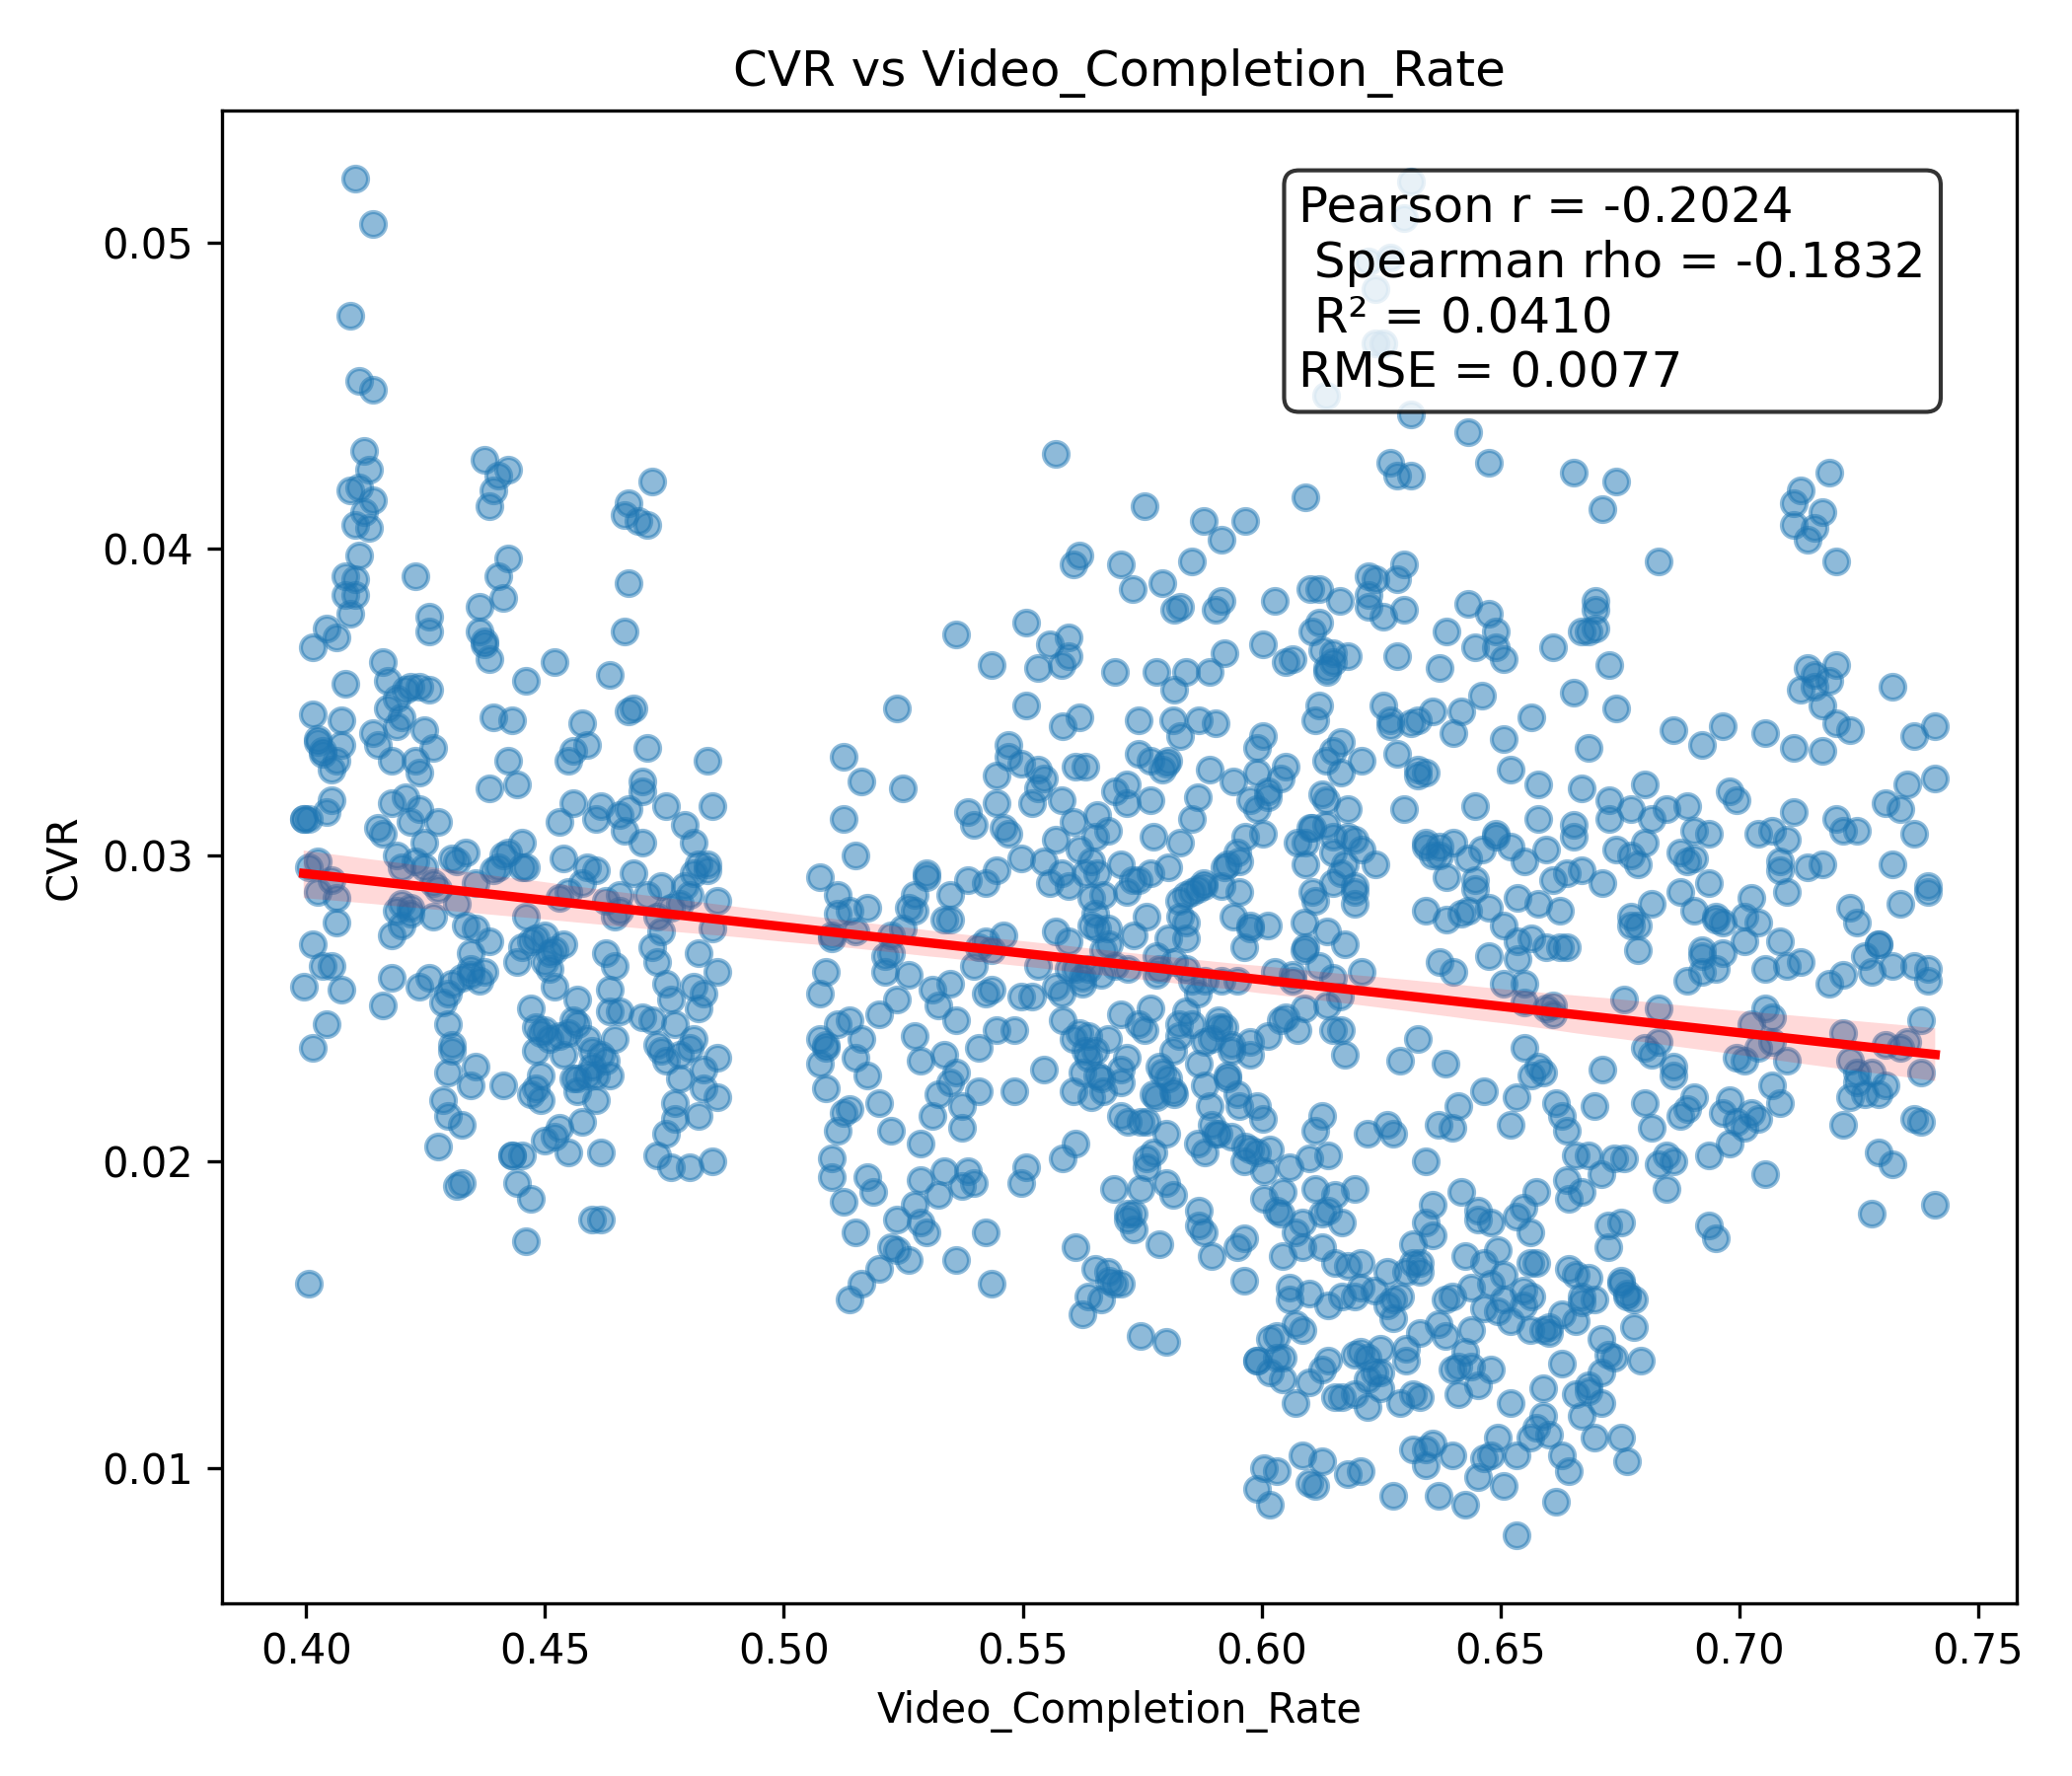
\includegraphics[width=0.7\textwidth]{images/CVR_vs_Video_Completion_Rate.png}
	\caption{CVR vs Video Completion Rate}
	\label{appendix:video_completion_rate}
\end{figure}

These results suggests that campaigns with higher video completion rates tend to exhibit slightly lower conversion rates. However, the magnitude of the relationship is weak, indicating that Video Completion Rate alone is not a strong predictor of Conversion rate.

\section{Relationship Between Video Completion Rate and Platform}
\label{appendix:video_completion_rate_platform_analysis}

\subsection{Video Completion Rate by Platform}
\label{appendix:video_completion_rate_platform_analysis_VCR}

\subsubsection{Descriptive Statistics}

\begin{table}[H]
	\centering
	\caption{Descriptive statistics for Video Completion Rate by platform.}
	\begin{tabular}{lcccc}
		\toprule
		Platform & Mean & Median & Std. Dev. & Count \\
		\midrule
		FB & 0.4430 & 0.4442 & 0.0250 & 299 \\
		TT & 0.6195 & 0.6163 & 0.0581 & 908 \\
		\bottomrule
	\end{tabular}
\end{table}

\subsubsection{Assumption Tests}

\subsubsection{Shapiro--Wilk Test}

\begin{table}[H]
	\centering
	\begin{tabular}{lc}
		\toprule
		Platform & p-value \\
		\midrule
		FB & $<0.0001$ \\
		TT & $<0.0001$ \\
		\bottomrule
	\end{tabular}
\end{table}

Both platform distributions significantly deviated from normality ($p<0.05$).

\vspace{0.3cm}

\subsubsection{Levene's Test}

\begin{table}[H]
	\centering
	\begin{tabular}{lc}
		\toprule
		Statistic & Value \\
		\midrule
		p-value & $<0.0001$ \\
		\bottomrule
	\end{tabular}
\end{table}

The variability of \textbf{Video Completion Rate differed significantly} between platforms. However, it is important to note that TT has 3 product\_categories while FB has 1, so the difference in STD may be attributed to TT having more diverse product categories.

\vspace{0.3cm}

\subsubsection{Kruskal--Wallis Test}

\begin{table}[H]
	\centering
	\begin{tabular}{lc}
		\toprule
		Statistic & Value \\
		\midrule
		H-statistic & 674.2412 \\
		p-value & $<0.0001$ \\
		\bottomrule
	\end{tabular}
\end{table}

The Kruskal--Wallis test indicates a statistically significant difference in Video Completion Rate between advertising platforms.

\vspace{0.3cm}

\subsubsection{Dunn Post-hoc Test}

\begin{table}[H]
	\centering
	\caption{Pairwise Dunn test p-values (Bonferroni adjusted).}
	\begin{tabular}{lcc}
		\toprule
		& FB & TT \\
		\midrule
		FB & -- & $<0.0001$ \\
		TT & $<0.0001$ & -- \\
		\bottomrule
	\end{tabular}
\end{table}

Facebook and TikTok exhibited statistically significant differences in Video Completion Rate, with TikTok achieving significantly higher completion rates than Facebook.

\subsubsection{Summary}

\begin{itemize}
	\item The \textbf{highest average Video Completion Rate} was achieved by \textbf{TikTok} (0.6195).
	\item The \textbf{lowest average Video Completion Rate} was observed for \textbf{Facebook} (0.4430).
	\item \textbf{TikTok achieved significantly higher Video Completion Rates than Facebook} ($p<0.05$).
\end{itemize}

\subsection{Video Completion Rate by TT Platform by Product Category}
\label{appendix:video_completion_rate_TT_platform_by_product}

\subsubsection{Descriptive Statistics}

\begin{table}[H]
	\centering
	\caption{Descriptive statistics for Video Completion Rate by product category.}
	\begin{tabular}{lcccc}
		\toprule
		Product Category & Mean & Median & Std. Dev. & Count \\
		\midrule
		Diet & 0.5618 & 0.5619 & 0.0320 & 293 \\
		Preworkout & 0.6181 & 0.6181 & 0.0349 & 300 \\
		Protein & 0.6745 & 0.6758 & 0.0387 & 315 \\
		\bottomrule
	\end{tabular}
\end{table}

\subsubsection{Assumption Tests}

\subsubsection{Shapiro--Wilk Test}

\begin{table}[H]
	\centering
	\begin{tabular}{lc}
		\toprule
		Product Category & p-value \\
		\midrule
		Diet & $<0.0001$ \\
		Preworkout & $<0.0001$ \\
		Protein & $<0.0001$ \\
		\bottomrule
	\end{tabular}
\end{table}

All product category distributions significantly deviated from normality ($p<0.05$).

\vspace{0.3cm}

\subsubsection{Levene's Test}

\begin{table}[H]
	\centering
	\begin{tabular}{lc}
		\toprule
		Statistic & Value \\
		\midrule
		p-value & 0.0001 \\
		\bottomrule
	\end{tabular}
\end{table}

The variability of \textbf{Video Completion Rate differed significantly} across product categories.

\vspace{0.3cm}

\subsubsection{Kruskal--Wallis Test}

\begin{table}[H]
	\centering
	\begin{tabular}{lc}
		\toprule
		Statistic & Value \\
		\midrule
		H-statistic & 587.1425 \\
		p-value & $<0.0001$ \\
		\bottomrule
	\end{tabular}
\end{table}

The Kruskal--Wallis test indicates statistically significant differences in Video Completion Rate across product categories.

\vspace{0.3cm}

\subsubsection{Dunn Post-hoc Test}

\begin{table}[H]
	\centering
	\caption{Pairwise Dunn test p-values (Bonferroni adjusted).}
	\begin{tabular}{lccc}
		\toprule
		& Diet & Preworkout & Protein \\
		\midrule
		Diet & -- & $<0.0001$ & $<0.0001$ \\
		Preworkout & $<0.0001$ & -- & $<0.0001$ \\
		Protein & $<0.0001$ & $<0.0001$ & -- \\
		\bottomrule
	\end{tabular}
\end{table}

All pairwise comparisons between product categories were statistically significant, indicating that each product category achieved a distinct level of Video Completion Rate.

\subsubsection{Within the TT Platform we have the following summary:}

\begin{itemize}
	\item The \textbf{highest average Video Completion Rate} was achieved by \textbf{Protein} (0.6745).
	\item The \textbf{lowest average Video Completion Rate} was observed for \textbf{Diet} (0.5618).
	\item \textbf{All product categories differed significantly} in Video Completion Rate ($p<0.05$), with Protein achieving the highest completion rates, followed by Preworkout and Diet.
\end{itemize}

\subsection{Video Completion Rate by Region}
\label{appendix:video_completion_rate_region_analysis_VCR}

\subsubsection{Descriptive Statistics}

\begin{table}[H]
	\centering
	\caption{Descriptive statistics for Video Completion Rate by region.}
	\begin{tabular}{lcccc}
		\toprule
		Region & Mean & Median & Std. Dev. & Count \\
		\midrule
		Midwest & 0.6206 & 0.6188 & 0.0584 & 220 \\
		Northeast & 0.6191 & 0.6165 & 0.0578 & 229 \\
		South & 0.6199 & 0.6160 & 0.0587 & 228 \\
		West & 0.6184 & 0.6140 & 0.0580 & 231 \\
		\bottomrule
	\end{tabular}
\end{table}

\subsubsection{Assumption Tests}

\subsubsection{Shapiro--Wilk Test}

\begin{table}[H]
	\centering
	\begin{tabular}{lc}
		\toprule
		Region & p-value \\
		\midrule
		Midwest & 0.0096 \\
		Northeast & 0.0090 \\
		South & 0.0028 \\
		West & 0.0065 \\
		\bottomrule
	\end{tabular}
\end{table}

All regional distributions significantly deviated from normality ($p<0.05$).

\vspace{0.3cm}

\subsubsection{Levene's Test}

\begin{table}[H]
	\centering
	\begin{tabular}{lc}
		\toprule
		Statistic & Value \\
		\midrule
		p-value & 0.9766 \\
		\bottomrule
	\end{tabular}
\end{table}

No statistically significant difference in the variability of \textbf{Video Completion Rate} was observed across regions.

\vspace{0.3cm}

\subsubsection{Kruskal--Wallis Test}

\begin{table}[H]
	\centering
	\begin{tabular}{lc}
		\toprule
		Statistic & Value \\
		\midrule
		H-statistic & 0.1893 \\
		p-value & 0.9793 \\
		\bottomrule
	\end{tabular}
\end{table}

The Kruskal--Wallis test indicates that there are no statistically significant differences in Video Completion Rate across regions.

\subsubsection{Summary}

\begin{itemize}
	\item The \textbf{highest average Video Completion Rate} was achieved by the \textbf{Midwest} (0.6206).
	\item The \textbf{lowest average Video Completion Rate} was observed for the \textbf{West} (0.6184).
	\item \textbf{No statistically significant differences} in Video Completion Rate were observed across regions ($p \geq 0.05$).
\end{itemize}

\subsection{Video Completion Rate by Competitive Event}
\label{appendix:video_completion_rate_competitive_event_analysis_VCR}

\subsubsection{Descriptive Statistics}

\begin{table}[H]
	\centering
	\caption{Descriptive statistics for Video Completion Rate by competitive event status.}
	\begin{tabular}{lcccc}
		\toprule
		Competitive Event & Mean & Median & Std. Dev. & Count \\
		\midrule
		False & 0.6189 & 0.6152 & 0.0580 & 872 \\
		True & 0.6335 & 0.6195 & 0.0610 & 36 \\
		\bottomrule
	\end{tabular}
\end{table}

\subsubsection{Assumption Tests}

\subsubsection{Shapiro--Wilk Test}

\begin{table}[H]
	\centering
	\begin{tabular}{lc}
		\toprule
		Competitive Event & p-value \\
		\midrule
		False & $<0.0001$ \\
		True & 0.0273 \\
		\bottomrule
	\end{tabular}
\end{table}

Both distributions significantly deviated from normality ($p<0.05$).

\vspace{0.3cm}

\subsubsection{Levene's Test}

\begin{table}[H]
	\centering
	\begin{tabular}{lc}
		\toprule
		Statistic & Value \\
		\midrule
		p-value & 0.9008 \\
		\bottomrule
	\end{tabular}
\end{table}

No statistically significant difference in the variability of \textbf{Video Completion Rate} was observed between competitive and non-competitive event periods.

\vspace{0.3cm}

\subsubsection{Kruskal--Wallis Test}

\begin{table}[H]
	\centering
	\begin{tabular}{lc}
		\toprule
		Statistic & Value \\
		\midrule
		H-statistic & 1.5983 \\
		p-value & 0.2061 \\
		\bottomrule
	\end{tabular}
\end{table}

The Kruskal--Wallis test indicates that there are no statistically significant differences in Video Completion Rate between competitive and non-competitive event periods.

\subsubsection{Summary}

\begin{itemize}
	\item The \textbf{highest average Video Completion Rate} was observed during \textbf{competitive events} (0.6335).
	\item The \textbf{lowest average Video Completion Rate} was observed during \textbf{non-competitive event periods} (0.6189).
	\item \textbf{No statistically significant difference} in Video Completion Rate was observed between competitive and non-competitive event periods ($p \geq 0.05$).
\end{itemize}

\begin{figure}[H]
	\centering
	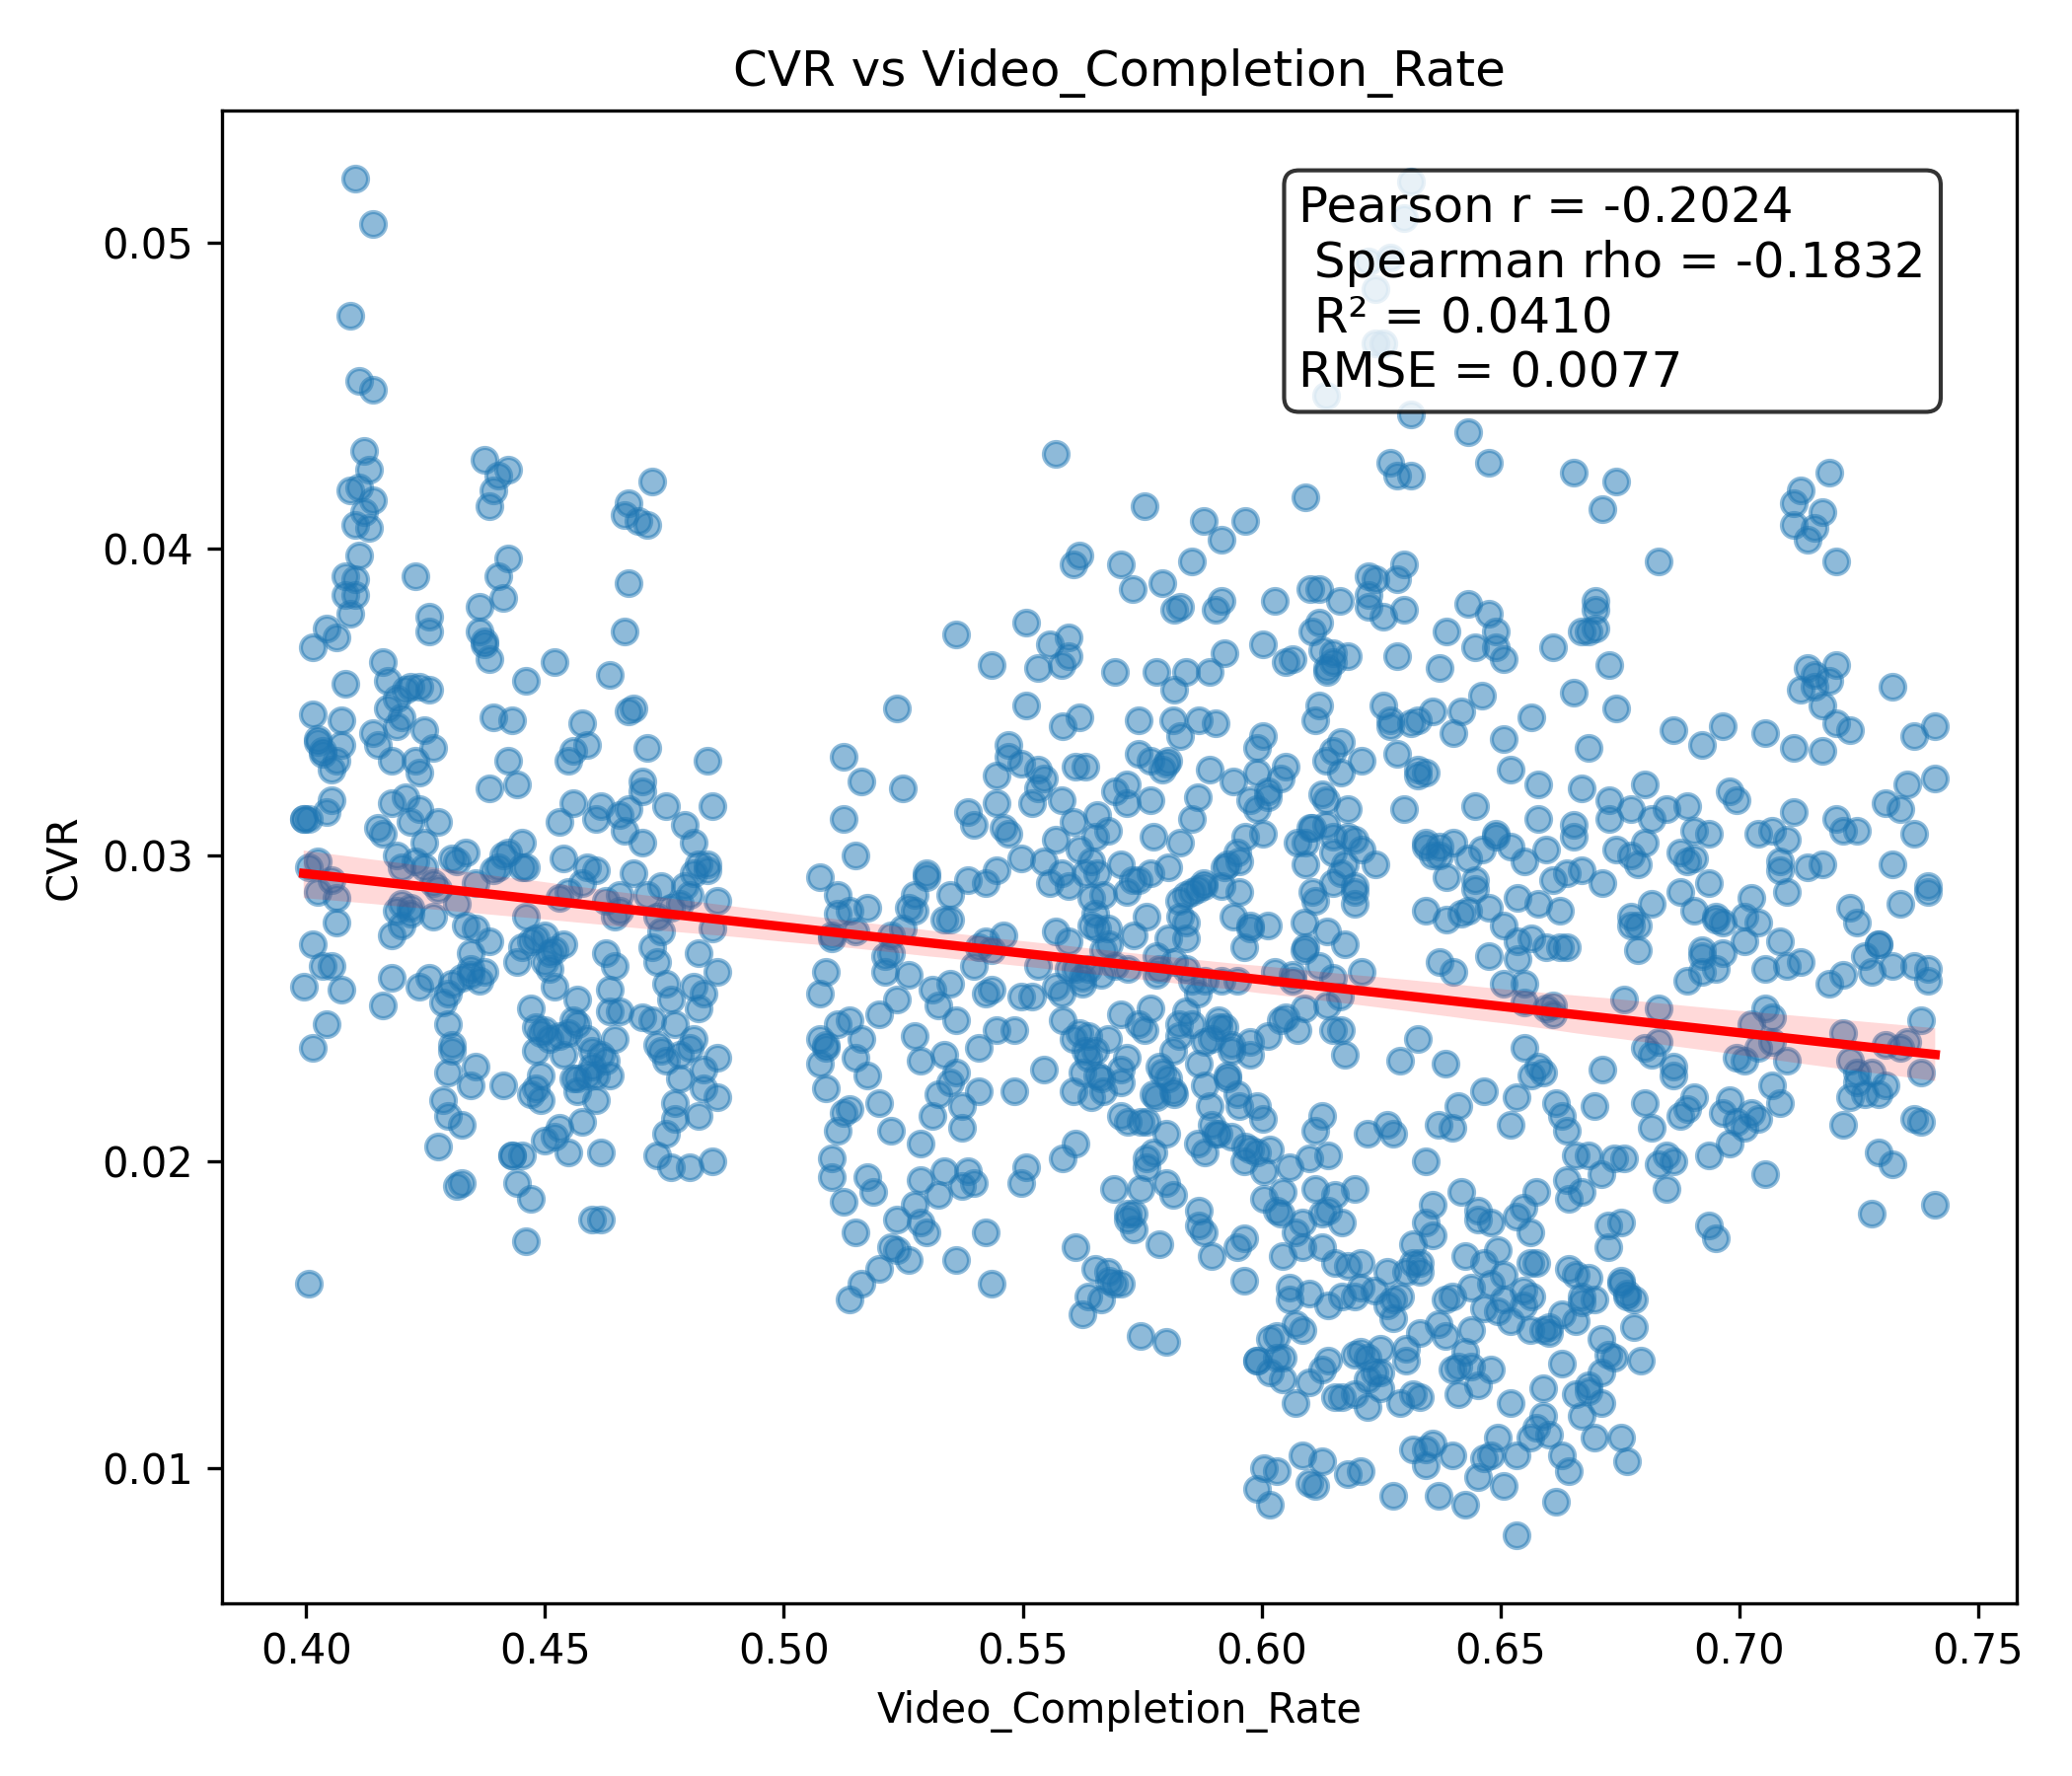
\includegraphics[width=0.7\textwidth]{images/CVR_vs_Video_Completion_Rate.png}
	\caption{CVR vs Video Completion Rate}
	\label{appendix:video_completion_rate_by_platfor}
\end{figure}



%\subsection{Video Com}
\subsection{Summary for Video Completion Rate by Platform}
\begin{figure}[H]
	\centering
	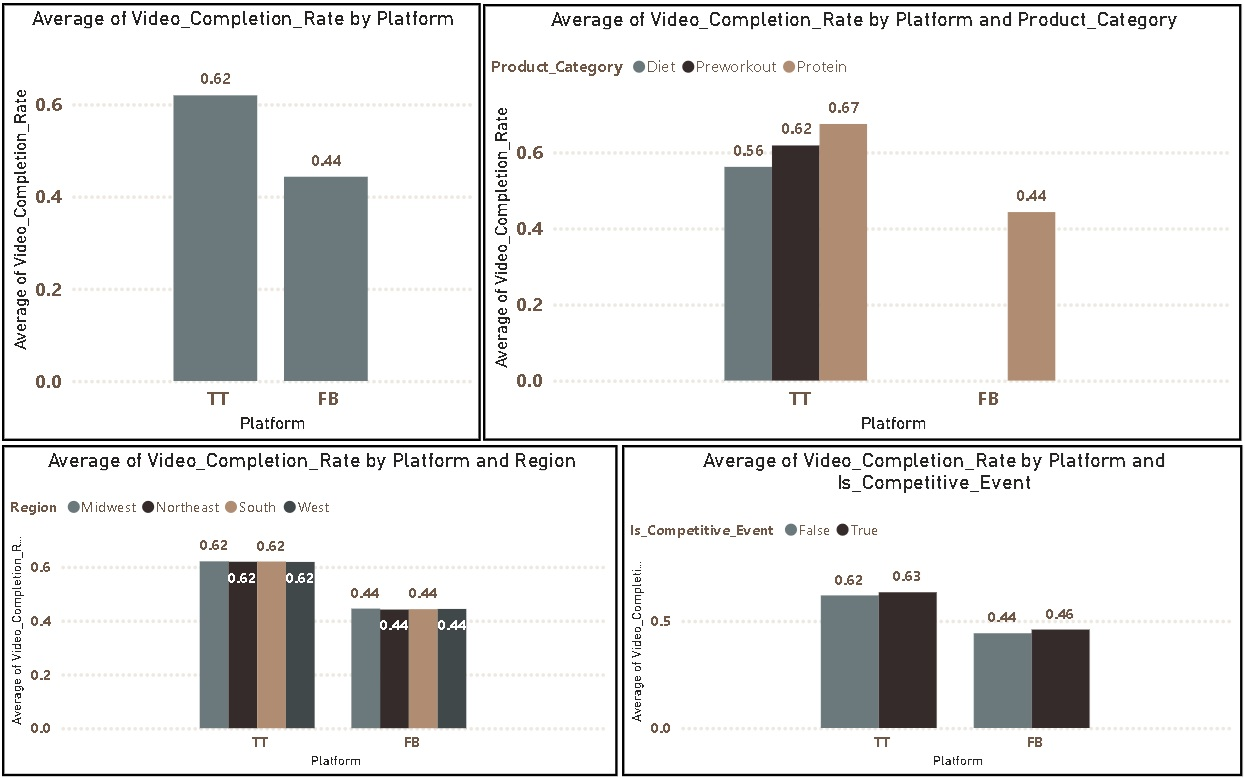
\includegraphics[width=1\textwidth]{images/video_completion_by_platform_by.jpg}
	\caption{Scatter plots of CVR versus Video Completion Rate grouped by platform, product category, competitive event status, and region}
	\label{fig:video_completion_rate_categorized}
\end{figure}

\begin{itemize}
	
	\item Video ads from TT platform exhibited higher video completion rate for Protein product category [Appendix \ref{appendix:video_completion_rate_platform_analysis_VCR}].
	
	\item Within the TT platform, product category seem to significantly affect video completion rate where Protein product exhibits the highest video completion rate [Appendix \ref{appendix:video_completion_rate_TT_platform_by_product}].
	
	\item Further tests, like FB video ads with Preworkout and Diet product categories are needed for evidence of Platform effects to video completion rate.
	
	\item Competitive events and Region seem to not affect the video completion rate across TT and FB Platforms.
\end{itemize}

Overall, product categories and platform(potentially) significantly affect video completion rate. These insights will be helpful for campaigns with a goal of maximizing video completion rate.



